\documentclass[preview]{standalone}


\usepackage{tikz}
\usetikzlibrary{arrows, automata, topaths, calc, shapes.geometric}

\begin{document}

\begin{figure}[h!]
    
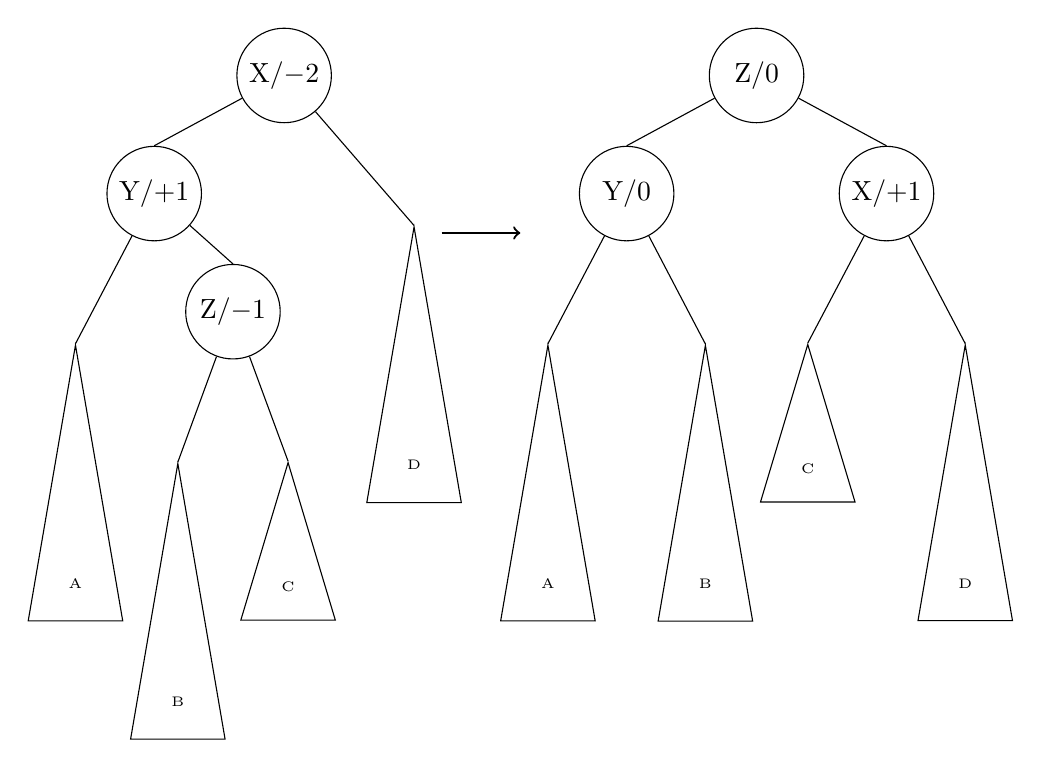
\begin{tikzpicture}[
    inner/.style={circle,draw,minimum width=12mm,inner sep=1pt},
    leaf/.style={isosceles triangle,draw,shape border rotate=90,isosceles triangle stretches=true, minimum height=20mm,minimum width=12mm,inner sep=0,yshift={-20mm},font=\tiny},
    large leaf/.style={leaf,minimum height=35mm,yshift={-14.5mm}},
    level 1/.style={sibling distance=33mm},
    level 2/.style={sibling distance=20mm},
    level 3/.style={sibling distance=14mm}]

    \node[inner] at (2,4)  {X/$-2$}
    [child anchor=north]
    child {node[inner] {Y/$+1$}
        child {node[large leaf] {A}}
        child {node[inner] {Z/$-1$}
        child {node[large leaf] {B}}
        child {node[leaf] {C}}}}
    child {node[large leaf] {D}};

    \draw[thick, ->] (4,2) -- (5,2);

    \node[inner] at (8,4)  {Z/$0$}
    [child anchor=north]
    child { node[inner] {Y/$0$} 
        child {node[large leaf] {A}}
        child {node[large leaf] {B}}}
    child {node[inner] {X/$+1$}
        child {node[leaf] {C}}
        child {node[large leaf] {D}}};
\end{tikzpicture}
\end{figure}
\end{document}
